\chapter{A prototype of a machine learning workflow to classify land use} \label{ch:ml_workflow}

The fourth phase of the CRISP-DM process model for data mining projects is modeling;
this chapter introduces a prototype of a machine learning workflow to classify land use from the housing market dynamics using the augmented Teranet dataset, production of which was described in chapter~\ref{ch:data_preparation}.
As was previously mentioned in section~\ref{sec:teranet_challenges_solution}, one of the major features missing from the available version of Teranet's dataset is the information about the type of property being transacted, which introduces a major limitation on how Teranet's data can be used.
As was described in chapter~\ref{ch:data_preparation}, parcel-level land use information from DMTI and the Department of Geography has been spatially joined to Teranet records, but these sources of land use information also have their limitations:

\begin{itemize}
    \item DMTI's land use data does not offer any split between subcategories of residential properties and only covers the period from 2001 to 2014
    \item land use data from the Department of Geography is a lot more detailed and accurate, but has been collected at a single point in time over the summer of 2012 and 2013
    \item neither of the available land use sources covers the full span of the Longitudinal Housing Market Research conducted by UTTRI (1986--2016)
\end{itemize}

To address this issue, detailed land use from the Department of Geography can be used as labelled data to train a machine learning model capable of recognizing certain property types that have characteristically different behavior on the housing market.
For example, the proposed model would be able to differentiate a detached house from a condo through such features as high / low volume of transactions, ratio of price to median price for that year, etc.
Chapter~\ref{ch:data_preparation} described the production of a dataset that combines the new features engineered from Teranet data with Census and TTS variables based on spatial and temporal relationships that were discussed in chapter~\ref{ch:spatial_and_temporal_relationships}.
In this chapter, this dataset is used to investigate the opportunity to implement a classification algorithm to determine the parcel land use at Teranet transaction level based on the housing market dynamics (land use is determined for each Teranet record, recognizing the changes of land use on the same parcel with time).
This way, a machine learning algorithm could provide a scalable solution to automate a labour-intensive task of collecting parcel-level detailed land use and expand the temporal span for which the land use data collected by the Department of Geography can be used with accuracy.

\section{Selecting and encoding the target variable} \label{sec:select_encode_target}

According to the results of an Exploratory Data Analysis (EDA), different property types have characteristically different behaviour on the housing market.
Figure~\ref{fig:xy_total_sales_dist_by_lu} shows the distributions of total count of Teranet records per coordinate pair by the 10 most frequently encountered land use categories used in the Department of Geography's dataset.

\begin{figure}[hbt!]
    \centering
    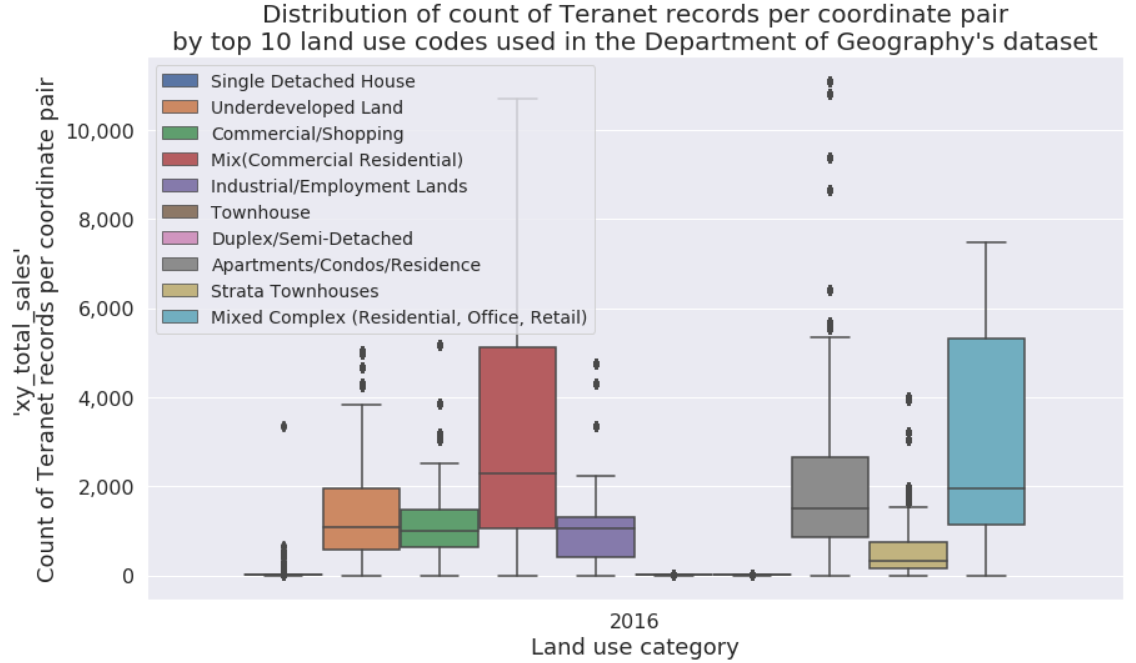
\includegraphics[width=0.98\linewidth,trim=0 0 0 0,clip]{xy_total_sales_dist_by_lu.png}
    \caption{Distributions of total count of Teranet records per coordinate pair by the top 10 land use categories.
    It can be seen that detached houses, duplexes, and townhouses (``collapsed" boxplots) have much lower numbers of records per coordinate pair.
    It can also be seen that there are some outliers present on the category of detached houses (first boxplot from the left).
    These outliers most likely represent mislabelled records, as it is very unlikely that a detached house can have almost 4,000 sales.}
    \label{fig:xy_total_sales_dist_by_lu}
\end{figure}

The target variable used for the purposes of investigating the possibility of land use classification using the housing market dynamics was constructed by reducing the land use codes found in the Department of Geography's land use dataset.
Department of Geography's land use categories that have the highest counts of Teranet records have been used to reduce all different property types to the three major land use classes.
Many machine learning algorithms are subject to a frequency bias in which they place more emphasis on learning from data observations which occur more frequently;
to address this, the three classes were selected to have a comparable number of Teranet records between themselves and thus produce a more balanced dataset.
In addition, the chosen groupings combine categories that have a similar distribution of price and count of sales per coordinate pair between land use categories that were grouped together to form a single class.
For example, detached and semi-detached houses and townhouses would have a much smaller frequency of transaction and a higher median price per coordinate pair when compared to condos and strata townhouses.
Figure~\ref{fig:class_2_price_dist} shows an example of such grouping: for target class 1, Duplex/Semi-Detached properties are grouped together with Townhouses;
together with Single Detached Houses the three categories form a single target class ``house''.

\vspace{5mm}

The three target classes that were introduced are:

\begin{itemize}
    \item Class 0: ``condo'', including Apartments/Condos/Residence and Strata Townhouses
    \item Class 1: ``house'', including Single Detached Houses, Duplex/Semi-Detached and Townhouses
    \item Class 2: ``other'', including Commercial/Shopping, Mix (Commercial Residential), Industrial/Employment Lands, and everything else
\end{itemize}

\begin{figure}[ht]
    \centering
    \begin{subfigure}{\linewidth}
        \centering
        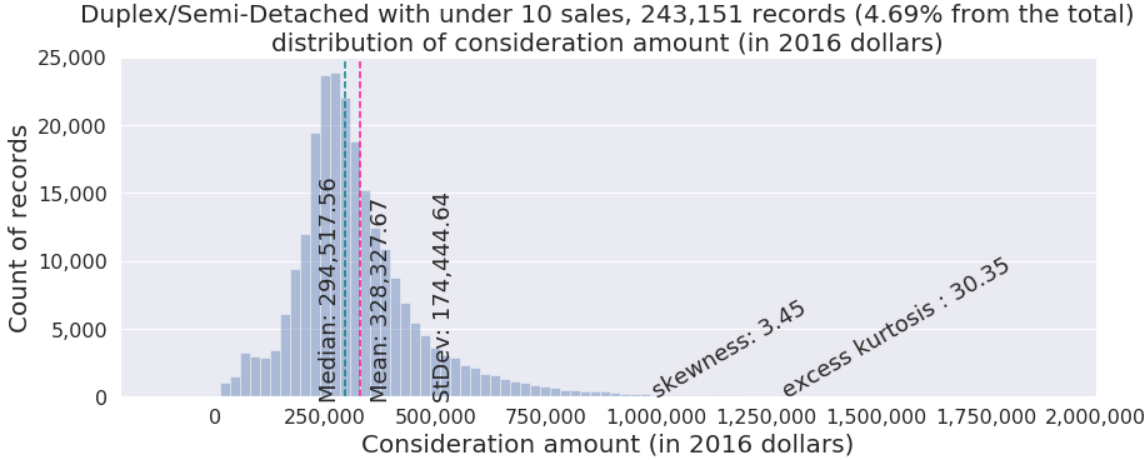
\includegraphics[width=.9\linewidth]{duplex_price_dist.png}
        \label{fig:duplex_price_dist}
        \caption{Duplex/Semi-Detached}
    \end{subfigure}

    \begin{subfigure}{\linewidth}
        \centering
        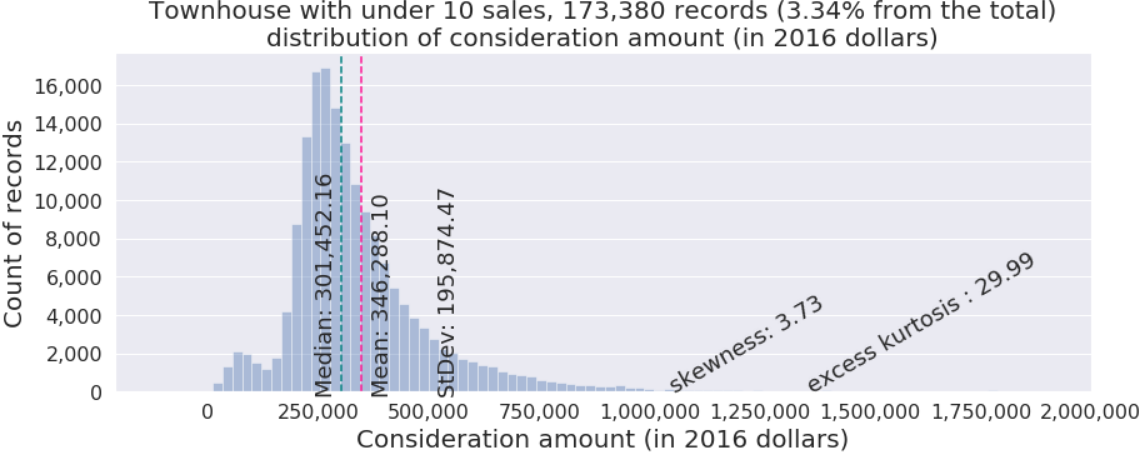
\includegraphics[width=.9\linewidth]{townhouse_price_dist.png}
        \label{fig:townhouse_price_dist}
        \caption{Townhouse}
    \end{subfigure}
    \caption{Distribution of price (in 2016 dollars) for two out of the three property types that are grouped together under Class 1: ``house''.
    Both categories have similar distributions of price and records per coordinate pair between themselves and with Single Detached Houses, and thus all three categories are grouped together to form a single target class ``house''.}
    \label{fig:class_2_price_dist}
\end{figure}

Classification algorithms, a subcategory of algorithms for supervised learning, predict the discrete unordered categorical class labels of new instances based on past observations.
A trained algorithm is capable of using a set of rules that were learned from past observations to distinguish the new instances between the possible classes.
Once the classes have been determined and assigned, the target variable must be encoded, as it is considered good practice to provide class labels as integer arrays to algorithms to avoid technical glitches and improve computational efficiency.
Class labels are not ordinal and classification estimators in the scikit-learn\cite{scikit-learn} machine learning library in Python treat them as categorical data that does not imply any order.

\section{Missing values} \label{sec:missing_values}

As was mentioned in section~\ref{sec:feature_engineering}, some of the new features engineered from Teranet attributes, such as `xy\_years\_since\_last\_sale' and `xy\_years\_to\_next\_sale' contain missing values in each case of the first or the last Teranet record coming from a coordinate pair.
Since classification algorithms cannot handle inputs with missing values, during classification these values were replaced using the following logic:

\begin{itemize}
    \item For all the records with missing `xy\_years\_since\_last\_sale' (first record from a coordinate pair), values were replaced with the median `xy\_years\_to\_next\_sale' for this subset (median time interval in years between all future sales from this Teranet subset).
    \item For all the records with missing `xy\_years\_to\_next\_sale' (last record from a coordinate pair), values were replaced with the median `xy\_years\_since\_last\_sale' for this subset (median time interval in years between all past sales from this Teranet subset).
\end{itemize}

This replacement affects a large number of Teranet records, as there are many coordinate pairs with a low count of transactions in the dataset.
At the same time, it allows the classification algorithm to work on the majority of Teranet data, which improves the generalization of the algorithm and allows classifying land use of most Teranet records.
As will be discussed in chapter~\ref{ch:model_evaluation}, features that have missing values also have strong predictive power for land use classes and thus are best kept in the input set with the missing values replaced.
This replacement is done during the fitting of classification algorithm and is not recorded in the final version of Teranet's dataset with new features and keys, where the missing values are left as missing.

\section{Dimensionality reduction} \label{sec:dimensionality_reduction}

Quality of the data plays a critical part in the success of application of a machine learning algorithm, and one of important aspects of data quality is the dimensionality of input space.
The input space may contain features that are either redundant or irrelevant;
highly correlated features also introduce multicollinearity and can make the model unstable, or too sensitive to small changes in the input data.
In machine learning, statistics, and information theory, dimensionality reduction is the process of reducing the number of random variables under consideration;
there is a number of reasons for reducing dimensionality of a dataset:

\begin{enumerate}
    \item reducing the number of features improves computational efficiency and reduces training times
    \item in case of a low signal-to-noise ratio in the dataset, dimensionality reduction can improve the predictive performance of an algorithm\cite{RaschkaMirjalili2017}
    \item simpler models are easier to interpret\cite{James2013}
    \item excessive complexity of the model could cause overfitting\cite{RaschkaMirjalili2017}
    \item the curse of dimensionality\cite{Bellman1954} (in the context of machine learning, the curse of dimensionality describes the phenomena where the feature space becomes too sparse for the size of the training dataset)\cite{RaschkaMirjalili2017}
\end{enumerate}

There is a number of approaches that could be utilized to reduce the dimensionality of the feature space.
There are two main categories of dimensionality reduction techniques:
\begin{itemize}
    \item feature selection, also referred to as Feature Subset Selection, or (FSS), where a subset of the original features is selected
    \item feature extraction, where a new feature subspace is constructed from information derived from the original feature set
\end{itemize}

Feature selection can either be performed manually or by utilizing a feature selection algorithm.
Exhaustive evaluation of all possible feature subsets is computationally unfeasible even for a moderate number of features.
For example, if we are given a feature set with $m = 64$ features and want to reduce it to $n = 11$, an exhaustive evaluation would involve over $10^{11}$ possible feature subsets:

\begin{equation}
    _{m}C_n = _{64}C_{11} = \binom{64} {11} = \frac{64!} {11!(64 - 11)!} = 743,595,781,824
\end{equation}

Feature selection algorithms present a practical approach to feature selection at scale;
such algorithms combine a search strategy for proposing new feature subsets with an objective function to evaluate these subsets;
objective function plays the role of a feedback signal used by the search strategy to choose between candidate subset.
Objective functions are divided into three major groups:

\begin{itemize}
    \item filters
    \begin{itemize}
        \item evaluate candidate feature subsets by their information content (e.g., inter/intra class distance, mutual information, etc.)
        \item advantages: have faster execution time since there generally is no iterative computation;
        have good generality since they evaluate the intrinsic properties of the data.
        \item disadvantages: tend to select large feature subsets due to monotonic objective functions
    \end{itemize}
    \item wrappers
    \begin{itemize}
        \item use a classifier to evaluate subsets by their predictive accuracy
        \item advantages: have better accuracy since they select subsets based on specific interactions between the classifier and the dataset
        \item disadvantages: slower to execute since a classifier needs to be re-trained multiple times;
        selected feature subset will be specific to the classifier that was used to evaluate the candidate subsets.
    \end{itemize}
    \item embedded methods
    \begin{itemize}
        \item feature selection is performed as a part of model construction process (i.e., LASSO method for constructing a linear model with L1 regularization)\cite{Scikit-learndevelopers2019}
    \end{itemize}
\end{itemize}

A combination of different FSS techniques was applied to reduce the dimensionality of the dataset with Teranet, TTS, and Census variables for classification from 64 to 11 input features.
The first method utilized was SelectFromModel in scikit-learn, a wrapper FSS algorithm that selects an optimal size and composition of a feature subset by fitting the provided classifier to training data and getting the importance weights from the fit model.
SelectFromModel with Random Forest classifier has determined the optimal number of features to be 18;
this number of features was provided to the other FSS algorithms to select the 18 best features from the dataset according to each method.

The second FSS method that was applied to the augmented Teranet dataset comes from the filter family of objective functions: a univariate feature selection algorithm SelectKBest in scikit-learn;
this method selects $k$ highest scoring features based on their scores on the specified univariate statistical test.
Univariate FSS techniques can be useful for better understanding of the data, as they examine each feature individually to determine the strength of its relationship with the target variable.
However, due to this fact, these methods will not necessarily result in improvement in the generalization of a learning algorithm, and thus their results have been used for feature selection in combination with other methods discussed in this section.
The following statistical tests from scikit-learn have been selected for scoring features using SelectKBest FSS algorithm:

\begin{itemize}
    \item Chi-squared stats of non-negative (pre-normalized) features for classification tasks
    \item ANOVA F-value between label/feature for classification tasks
    \item Mutual information for a discrete target
\end{itemize}

The third family of FSS algorithms that were applied were the recursive feature elimination algorithms, wrapper algorithms that evaluate candidate feature subsets and recursively eliminate features until the desired number of dimensions is reached.
RFE class in scikit-learn facilitates feature ranking with recursive feature elimination using the provided external classifier that assigns weights to features.
A more exhaustive approach to recursive feature elimination is the use of a sequential feature selection algorithm.
Sequential feature selection algorithms are a family of greedy search algorithms that are used to reduce an initial $d$-dimensional feature space to a $k$-dimensional feature subspace where $k<d$.

\begin{figure}[hbt!]
    \centering
    \begin{subfigure}[t]{.45\textwidth}
        \centering
        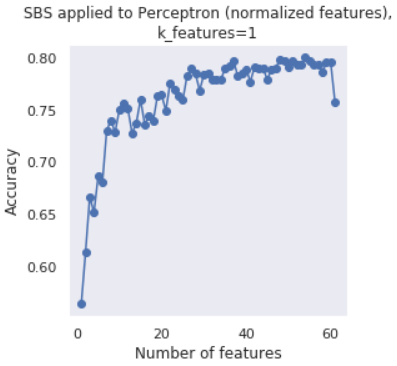
\includegraphics[width=\columnwidth,trim=0 0 0 0,clip]{sbs_perceptron.png}
        \caption{Perceptron}
        \label{fig:sbs_perceptron}
    \end{subfigure}
    ~ %add desired spacing between images, e. g. ~, \quad, \qquad, \hfill etc.
    %(or a blank line to force the subfigure onto a new line)
    \begin{subfigure}[t]{.53\textwidth}
        \centering
        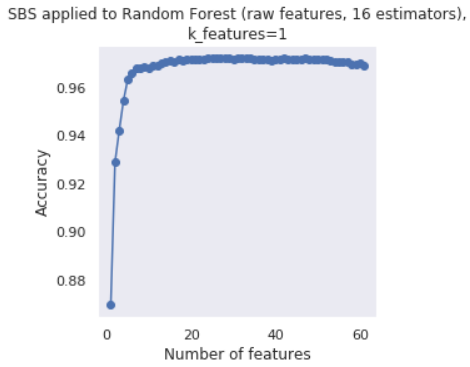
\includegraphics[width=\columnwidth,trim=0 0 0 0,clip]{sbs_forest.png}
        \caption{Random Forest}
        \label{fig:sbs_forest}
    \end{subfigure}
    \caption{Sequential Backward Selection (SBS) is a classic sequential FSS algorithm;
    on each iteration, it eliminates the feature that results in the minimum drop in performance of the provided classifier.
    Figure~\ref{fig:sbs_perceptron} shows SBS run on augmented Teranet dataset with Perceptron and figure~\ref{fig:sbs_forest} shows SBS with Random Forest.
    It can be seen that many features can be eliminated without a significant drop in performance of both classifiers, especially in the case of Random Forest.}
    \label{fig:sbs_teranet}
\end{figure}

Sequential Backward Selection (SBS) is a classic sequential FSS algorithm which aims to reduce the dimensionality of the initial feature subspace with a minimum decay in performance of the classifier;
in some cases of model overfitting, SBS can even improve the predictive power of a classifier.
On each iteration, a feature is removed using the defined criterion function $J$ that we want to minimize;
$J$ can simply be defined as the difference in performance of the classifier before and after the elimination of a particular feature.
Figure~\ref{fig:sbs_teranet} presents plots produced by running SBS algorithm on augmented Teranet dataset with Perceptron and Random Forest;
Sequential Backward Selection algorithm implemented as a Python class by Raschka and Mirjalili\cite{RaschkaMirjalili2017} has been used for this thesis.

\begin{figure}[hbt!]
    \centering
    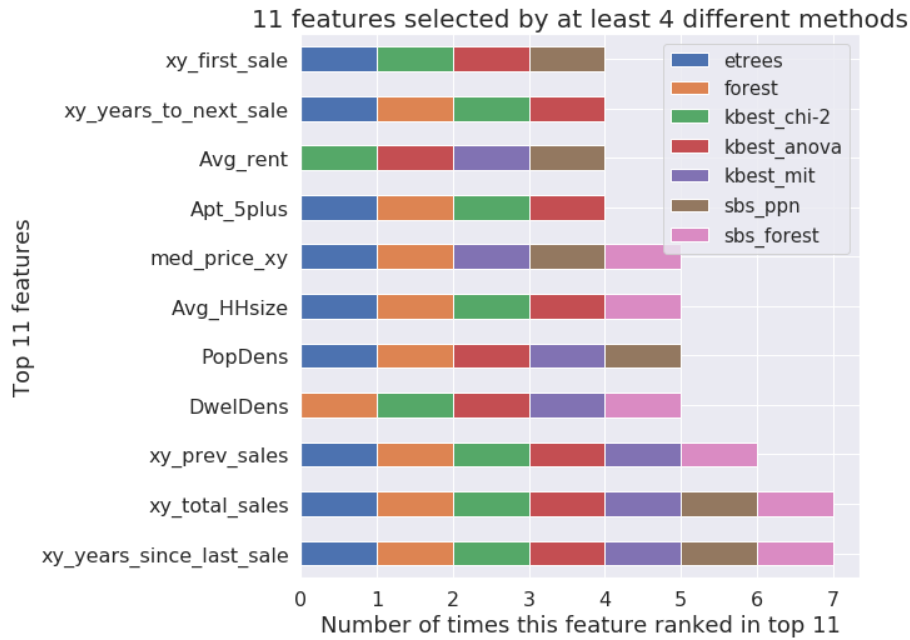
\includegraphics[width=0.7\linewidth,trim=0 0 0 0,clip]{top11f_selection_summary.png}
    \caption{FSS results: 11 features that were selected by at least four different feature selection methods.
    These features were used to select the best-performing model and make the final classification of land use of Teranet records.}
    \label{fig:top_feats}
\end{figure}

As can be seen from the plots produced by SBS, most features in the augmented Teranet dataset can be eliminated without a significant drop in performance of both linear and tree-based models.
As such, the final set of features to be used for land use classification was selected by combining the feature subsets selected by each of the FSS methods described above.
Features that have been selected by at least four different methods were selected as the final feature subset that was tested with the classification algorithms and used for final classification of land use;
figure~\ref{fig:top_feats} presents the 11 features that were selected using this logic: these are the 11 features that were selected by at least four different FSS techniques.

From the perspective of embedded feature selection methods, another possible approach to reduce the complexity of a model is to use L1 regularization to penalize large individual weights.
L1 regularization introduces a penalty term to the cost function which is taken as the norm of the weight vector defined as:

\begin{equation} \label{eq:l1_regularization}
    L1:~\norm{\vect{w}}_1 = \sum \limits_{j=1}^m \abs{w_j}
\end{equation}

L1 regularization is similar to L2 regularization, which is defined as:

\begin{equation} \label{eq:l2_regularization}
    L2:~\norm{\vect{w}}_2^2 = \sum \limits_{j=1}^m w_j^2
\end{equation}
where $m$ is the number of features.

However, since in the case of L1 regularization, the sum of squares of weights is replaced with the sum of the absolute values of weights, L1 regularization usually yields sparse feature vectors, since most feature weights will be zero\cite{RaschkaMirjalili2017,Scikit-learndevelopers2019}.
Sparsity of feature vectors can help us get rid of irrelevant features in a high-dimensional dataset;
in this context, L1 regularization can be understood as a technique for feature selection\cite{RaschkaMirjalili2017}.
L1 regularization was attempted with Logistic Regression and Linear Support Vector Classifier models in scikit-learn, but did not result in a significant improvement in model performance.

\section{Tuning model hyperparameters} \label{sec:tuning_hyperparameters}

One of the critical aspects of evaluating the performance of a machine learning model is the assessment of the algorithm's ability to not only perform well on the data that was used to train it, but also to generalize well to unseen, or test, data.
Evaluating the model on the same dataset that was used to train it will result in the optimistically biased estimate of the predictive power of a classifier;
hence the need to split the dataset into separate training and test subsets.
Comparing predictions made by the algorithm to true labels in the test subset can be understood as the unbiased performance evaluation of the model\cite{RaschkaMirjalili2017};
in this context, bias refers to the difference between the expected prediction accuracy of a model and its true prediction accuracy\cite{Raschka2018}.

To facilitate this, all GTHA Teranet records from 2011 to 2014 have been split into two subsets using random subsampling: 70\% of the data was used to train models and tune their hyperparameters, while 30\% of the data has been used as a test subset for the unbiased performance evaluation of the classifier.
Train and test subsets have been stratified across the target classes:
in this context, stratification means that training and test subsets will have the same proportions of class labels as the input dataset.

\begin{figure}[hbt!]
    \centering
    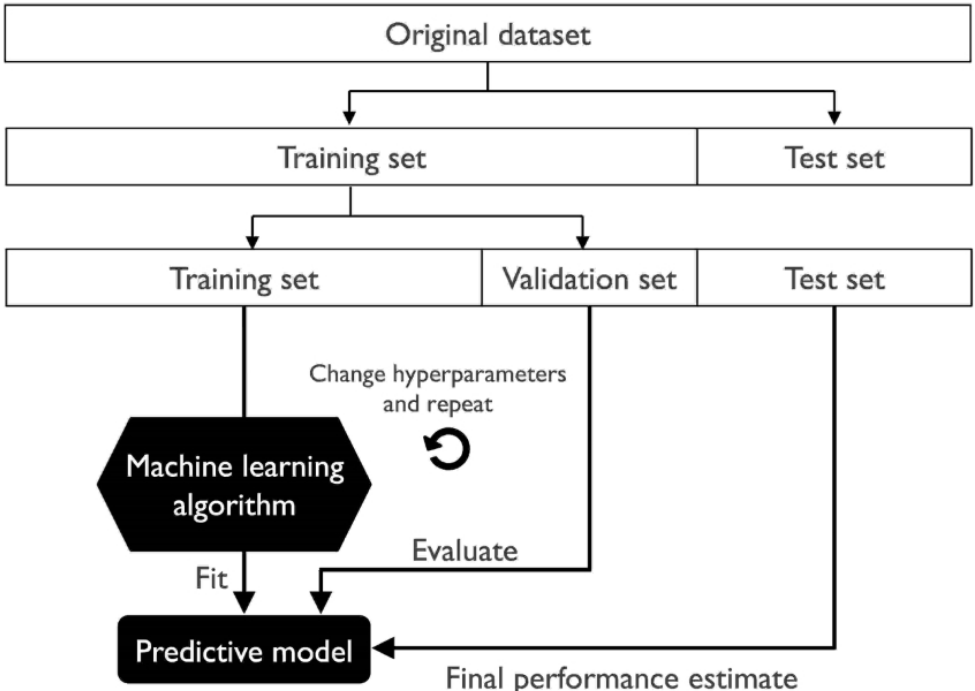
\includegraphics[width=0.7\linewidth,trim=0 0 0 0,clip]{holdout_validation_workflow.png}
    \caption{Holdout validation of a machine learning model as summarized by Raschka and Mirjalili\cite{RaschkaMirjalili2017}.}
    \label{fig:holdout_validation_workflow}
\end{figure}

There are two types of parameters in machine learning: those that are learned by parametric models from training data (i.e., weights in logistic regression), and the parameters that tune the performance of a learning algorithm, or its hyperparameters (i.e., regularization parameter in logistic regression or maximum depth of a decision tree).
If a model is too simple, it can suffer from underfitting and show poor performance on both the training and the test data (have high bias;
the bias of a learning algorithm is the persistent error that it is expected to make when trained on a given sample size\cite{Dietterich1995}).
On the other hand, if a model is too complex, it can overfit the training data and have poor generalization on test data (have high variance;
the variance captures the random variation in the algorithm from one training set to another\cite{Dietterich1995}).
An acceptable bias-variance trade-off can be found by tuning the hyperparameters of a learning model, but care must be taken to ensure unbiased assessment of its generalization performance.

There are no hard-and-fast rules that guarantee the best performance of a classifier on a given dataset\cite{Raschka2018};
thus, it becomes important to evaluate the performance of a classifier with different hyperparameters to find the best model settings prior to using the model to make predictions.
However, when evaluating different hyperparameters for estimators, there is a risk of overfitting on the test set because knowledge about the test set can ''leak'' into the model;
evaluation metrics will no longer report on generalization performance.
To address this issue, yet another part of the dataset can be held out as a so-called ''validation set'': training proceeds on the training set, with model hyperparameters being evaluated by its performance on the validation set;
when the experiment seems to be successful, final evaluation can be done on the test set.
Figure~\ref{fig:holdout_validation_workflow} presents an example of a workflow for tuning and evaluating a machine learning model using hold-out validation, as summarized by Raschka and Mirjalili\cite{RaschkaMirjalili2017}.

\begin{figure}[hbt!]
    \centering
    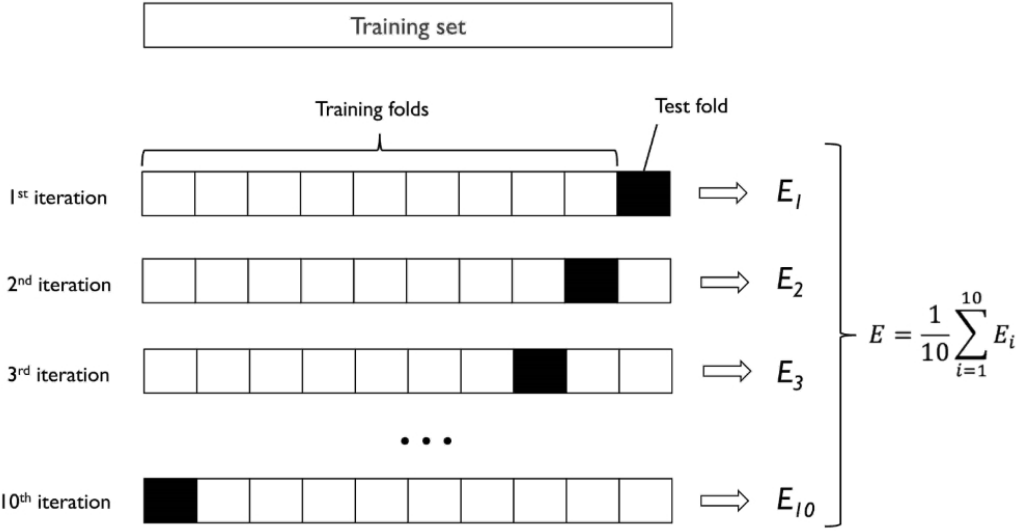
\includegraphics[width=0.9\linewidth,trim=0 0 0 0,clip]{kfold_validation_workflow.png}
    \caption{$k$-fold cross-validation as summarized by Raschka and Mirjalili\cite{RaschkaMirjalili2017}.
    In the case of $k=10$, the training dataset is divided into 10 folds, and during the 10 iterations, nine folds are used for training, and one fold is used as the test set for the model evaluation.
    Estimated performances (for example, classification accuracy or error) for each fold are then used to calculate the estimated average performance $E$ of the model.}
    \label{fig:kfold_validation_workflow}
\end{figure}

There is a shortcoming in this approach: by partitioning the available data into three sets, the number of samples which can be used for learning the model is drastically reduced;
results can depend on a particular random choice of the train and validation sets.
A solution to this problem is a procedure called cross-validation (CV for short): validation set is produced from the training set using such techniques as $k$-fold CV, while the test subset of data unseen by the model is held out for its final evaluation.
In a basic approach called $k$-fold CV, the training set is split into $k$ smaller sets and on each of $k$ iterations a model is trained using $k-1$ of the folds as training data;
the resulting model is validated on the held-out test fold of the data through such performance metrics as model accuracy.
The performance measure reported by $k$-fold cross-validation is then the average of the values computed in the loop.
Figure~\ref{fig:kfold_validation_workflow} presents $k$-fold cross-validation workflow to evaluate model performance as summarized by Raschka and Mirjalili\cite{RaschkaMirjalili2017}.

This approach can be computationally expensive, but does not waste too much data, as is the case when fixing an arbitrary validation set.
Empirical evidence shows that a good standard value for $k$ in $k$-fold cross-validation is 10, as seen in experiments conducted by Kohavi on various real-world datasets\cite{Kohavi1995}.
A slight further improvement in bias and variance estimates over the standard $k$-fold cross-validation can be achieved by using stratified $k$-fold cross-validation, as shown in the study conducted by Kohavi.
In stratified cross-validation, the class proportions are preserved in each fold to ensure that each fold is representative of the class proportions in the training dataset.
For this thesis, stratified $k$-fold cross-validation workflow has been used to tune model hyperparameters via grid search before the final evaluation of model performance was done using the held-out test set;
model evaluation results will be discussed in chapter~\ref{ch:model_evaluation}, examples of validation curves for decision tree and random forest are presented on figure~\ref{fig:validation_curves}.

\section{Feature scaling} \label{sec:feature_scaling}

Many machine learning algorithms are designed with the assumption that each feature takes values close to zero or, more importantly, that all features vary on comparable scales\cite{Scikit-learndevelopers2019b}.
Raw data rarely comes in the form and shape that is necessary for the optimal performance of a learning algorithm, and thus data preprocessing via scaling is one of the most crucial steps in machine learning workflows\cite{RaschkaMirjalili2017}.
Bringing different variables to the same scale can be accomplished by such techniques as standardization or normalization;
in addition, outliers that are present in data can be addressed by using non-linear transformations, such as quantile or power transforms.

\vspace{5mm}

The following preprocessing methods have been tested on the training dataset:

\begin{itemize}
    \item standardization (mean removal and variance scaling)
    \item normalization (min-max scaling to a range of [0, 1])
    \item max-abs (scale to a range of [-1, 1], maximum absolute value of each feature is scaled to unit size)
    \item robust scaling (more robust estimates for data with outliers)
    \item power transform (Yeo-Johnson, mapping to a Gaussian distribution)
    \item quantile transform (mapping to a Gaussian distribution)
    \item quantile transform (mapping to a uniform distribution)
    \item sample-wise L2 transform (normalize samples individually to unit norm)
\end{itemize}

All these preprocessing techniques were tested with classification algorithms for prediction accuracy and fit times;
results will be presented in chapter~\ref{ch:model_evaluation}.
It is important to note that the parameters for the previously mentioned procedures, such as feature scaling and dimensionality reduction, are solely obtained from the training dataset, and the same parameters are later reapplied to transform the test dataset and the full Teranet dataset for the final classification of land use;
this way, an unbiased estimate of model generalization can be obtained.

\section{Model selection} \label{sec:model_selection}

An important point to be summarized from the famous No Free Lunch Theorems (NFL)\cite{Wolpert1996,Wolpert1997} by David H. Wolpert is that no single classifier works best across all possible scenarios, as there is a lack of a priori distinctions between learning algorithms.
In practice, it is essential to compare the performance of at least a handful of different classification algorithms, since each of them has its inherent biases, in order to select the best performing model.
No single classification model enjoys superiority if we don't make any assumptions about the form of the function that maps input features to target variables and how this function can be learned\cite{RaschkaMirjalili2017}.

There are several possible ways of categorizing machine learning algorithms;
one of them is to separate algorithms into parametric and non-parametric models.
In parametric models, such as logistic regression, perceptron or linear Support Vector Machine (SVM), model parameters are estimated from the training set to learn a function that allows classifying new data without the need for the original training set, once the model has been fit.
In addition, the number of model parameters is fixed and does not change with the size of the training data.
In contrast, non-parametric models, such as instance-based learning models like $k$-Nearest Neighbors, can't be characterized by a fixed set of parameters, and the number of parameters grows with the amount of training data.

Another way of categorizing the algorithms that were used in this thesis is into linear, tree-based, and nearest neighbors model classes.
Models from the following three main classes of classification algorithms have been tested with the augmented Teranet dataset:

\begin{itemize}
    \item Linear models

    Linear models are used by a popular and broad class of procedures for solving classification tasks.
    These models aim at dividing the feature space into a collection of regions labelled according to the values that the target can take, where the decision boundaries between those regions are linear hyperplanes.
    Examples include:

    \begin{itemize}
        \item Perceptron learning algorithm

        Perceptron is a simple classification algorithm suitable for large-scale learning that was introduced by Frank Rosenblatt\cite{Rosenblatt1957a} in 1957 based on the McCulloch-Pitts (MCP) artificial neuron model\cite{McCulloch1990a} that was introduced in 1943.
        It is a parametric non-regularized model that only updates its weights on wrong predictions that it makes.

        \item Logistic Regression (L2, L1 regularization)

        Another simple yet more powerful parametric algorithm for linear and binary classification problems is logistic regression;
        it can also be expanded to multi-class problems through such techniques as One-versus-All (OvA).
        Logistic regression models the probabilities of an observation belonging to each of the $K$ classes via linear functions and is typically estimated by maximum likelihood.
        It is often used as an inference tool to understand the role of input variables in explaining the target, since it produces easily interpretable coefficients;
        in addition, it can also have significant predictive power in the cases when target classes are linearly separable\cite{RaschkaMirjalili2017}.

        \item Linear Discriminant Analysis

        Linear Discriminant Analysis (LDA) is most commonly used as a dimensionality reduction technique, but it can also have some practical uses as a classifier by itself.
        LDA assumes that the joint densities of all features given target's classes are multivariate Gaussians with the same covariance for each class.

        \item Quadratic Discriminant Analysis

        Quadratic Discriminant Analysis (QDA) is a classifier with a quadratic decision boundary;
        it relaxes the common covariance assumption of LDA through estimating a separate covariance matrix for each class.

        \item Linear Support Vector Classification (L2, L1 regularization)

        Support Vector Machines (SVM) represent another family of powerful and widely used algorithms used for maximum margin classification: optimization objectives for SVMs is to maximize the margin instead of minimizing the classification error.
        The margin is defined as the distance between the separating hyperplane (decision boundary) and the training samples that are closest to this hyperplane, which are the so-called support vectors\cite{RaschkaMirjalili2017}.

        \item Naive Bayes Classifier

        A Naive Bayes Classifier is a probabilistic classification technique based on Bayes Theorem with an assumption of independence among input features.
        It determines the probability that an example belongs to some class, calculating the probability that an event will occur given that some input event has occurred.
        These algorithms are computationally efficient and suitable for large datasets, but have the disadvantage of the assumption about the independence of input features.

    \end{itemize}

    \item Tree-based models

    Decision tree classifiers are attractive models due to their predictive power, computational efficiency and interpretability.
    In addition, these models are scale-invariant and require less data preprocessing.
    These models construct a flow-chart-like decision tree by learning simple decision rules similar to asking a series of questions, or in other words, introduce a set of boolean conjunctions.
    Examples include:

    \begin{itemize}

        \item Decision Tree Classifier

        Decision trees can build complex decision boundaries by dividing the feature space into rectangles by learning a series of questions to infer the class labels of the samples;
        questions are selected to maximize Information Gain (IG) on each split of the tree, defined as the difference in selected impurity measure (Gini, entropy, or classification error) between parent and child nodes.
        Splitting procedure is repeated until all the leaves are pure (consist of samples belonging to the same target class), or until selected maximum depth of the tree is reached.

        \item Random Forest Classifier

        High variance plays a more important role in poor performance of decision trees rather than high bias;
        thus, ensemble methods based on voting can improve their performance since voting methods are capable of reducing variance of a learning algorithm\cite{Dietterich1995}.
        Decision trees can be unstable due to small variations in the data, and a more robust approach is to combine multiple trees into an ensemble model.
        Random forest is a hugely popular classification algorithm due to its good classification performance, scalability, and ease of use\cite{RaschkaMirjalili2017}.
        Random forest averages multiple (deep) decision trees each of which individually suffers from high variance, to build a model with better generalization performance and less susceptible to overfitting.
        Prediction of the class label is aggregated by a majority vote from the selected number of trees, each of which is trained on a bootstrapped sample of records using a randomly selected subset of features.

    \end{itemize}

    \item Nearest Neighbors


    Neighbors-based classification presents a type of instance-based non-parametric learning: it does not attempt to construct a discriminative function to classify the target variable;
    instead, it simply stores instances of the training data.
    The principle behind nearest neighbors is to find a predefined number of training samples closest in distance to the new point, and predict the target label of a new sample using the majority vote of its neighbors.
    The number of samples can either be a user-defined constant ($k$-nearest neighbor learning), or vary based on the local density of points (radius-based neighbor learning).
    Commonly used distance metrics include Manhattan and Euclidean distance.

    \begin{itemize}

        \item $k$-Nearest Neighbors Classifier

        $k$-Nearest Neighbors classifier is a distance-based classification algorithm that uses a predefined number of samples considered as neighbors to each new point according to the selected distance metrics (Manhattan, Euclidean distances are a common choice).
        Class label of each new point is assigned by the majority vote of its neighbors.
        Number of neighbors $k$ and distance metric are the hyperparameters of a $k$-NN model.

    \end{itemize}

\end{itemize}

In order to compare different models, metrics to measure performance needed to be established, which will be discussed in section~\ref{sec:model_metrics}.
Results of model evaluation are presented in chapter~\ref{ch:model_evaluation}.

\section{Chapter summary} \label{sec:ml_workflow_summary}

One of the major features missing from Teranet's dataset is land use information covering a period of time starting from 1985.
This chapter introduced a prototype of machine learning workflow to classify land use at Teranet transaction level from housing market dynamics as reflected by augmented Teranet variables.
Such topics as methodology for feature selection, filling of the missing values, feature scaling, model hyperparameter tuning, unbiased assessment of model performance via such techniques as train-test split and $k$-fold cross-validation and selection of learning algorithms to be tested have been discussed in this chapter.
Chapter~\ref{ch:model_evaluation} presents the evaluation of model performance.